\documentclass[10pt, aspectratio=169]{beamer}

% --- 1. СТИЛЬ (BEAVER - White & Red) ---
% \usetheme{Madrid}           % Структура (блоки, отступы)
\usecolortheme{beaver}      % Цветовая схема (Белый/Серый/Красный)

% Твои настройки из запроса:
\beamertemplatenavigationsymbolsempty
\setbeamertemplate{blocks}[rounded=true, shadow=true]
\setbeamertemplate{footline}[frame number] % Номер страницы внизу

% Настройка шрифтов (сделаем чуть современнее стандартного)
% \usepackage{helvet}
% \renewcommand{\familydefault}{\sfdefault}

% --- 2. ПАКЕТЫ ---
\usepackage{graphicx}
\usepackage{booktabs}
\usepackage{algorithm}
\usepackage{algpseudocode}
\usepackage{amsmath}
\usepackage{caption}
\usepackage{xcolor}

% --- 3. ЦВЕТА ДЛЯ КОДА И АЛГОРИТМОВ ---
% Подгоняем под стиль Beaver (темно-красный и серый)
\definecolor{BeaverRed}{RGB}{204, 0, 0}       % Основной красный
\definecolor{BeaverGray}{RGB}{64, 64, 64}     % Темно-серый
\definecolor{CodeBg}{HTML}{F8F9FA}            % Светлый фон для блоков

% Настройка цветов алгоритма
\algrenewcommand\algorithmicrequire{\textbf{\textcolor{BeaverRed}{Input:}}}
\algrenewcommand\algorithmicensure{\textbf{\textcolor{BeaverRed}{Output:}}}
\algrenewcommand\algorithmicwhile{\textbf{\textcolor{BeaverRed}{while}}}
\algrenewcommand\algorithmicfor{\textbf{\textcolor{BeaverRed}{for}}}
\algrenewcommand\algorithmicif{\textbf{\textcolor{BeaverRed}{if}}}
\algrenewcommand\algorithmicreturn{\textbf{\textcolor{BeaverRed}{return}}}
\algrenewcommand\algorithmiccomment[1]{\hfill \textcolor{gray}{\# #1}}

% --- ИНФО ---
\title{Hyperband: A Novel Bandit-Based Approach to
Hyperparameter Optimization}
\subtitle{Lisha Li, Kevin Jamieson, Giulia DeSalvo, Afshin Rostamizadeh, Ameet Talwalkar}
\author{Talk by Dmitrii Vasilenko}
\date{}

\begin{document}

\maketitle

\begin{frame}{Problem Statement}
    \textbf{The Challenge:}
    \begin{itemize}
        \item Modern ML models (e.g., Deep Learning) take days/weeks to train.
        \item Performance critically depends on hyperparameters (LR, batch size, architecture).
    \end{itemize}

    \vspace{0.5cm}
    \textbf{Existing Solutions:}
    \begin{itemize}
        \item \textbf{Random Search:} Simple, parallelizable, but wastes resources fully training bad configurations.
        \item \textbf{Bayesian Optimization (SMAC, TPE, Spearmint):}
              \begin{itemize}
                  \item Focuses on \textit{selecting} the best config.
                  \item Computationally expensive in high dimensions.
                  \item Doesn't natively support early stopping.
              \end{itemize}
    \end{itemize}
\end{frame}

\begin{frame}{Mapping to Bandit Problems}
    The authors formulate HPO as a \textbf{Pure-Exploration Non-Stochastic Infinite-Armed Bandit} problem.

    \begin{block}{The Mapping}
        \begin{itemize}
            \item \textbf{Arms} = Hyperparameter configurations (sampled from a distribution).
            \item \textbf{Pulling an arm} = Allocating a resource (iteration, epoch, data subset).
            \item \textbf{Reward} = Validation loss (we want to minimize specific loss).
        \end{itemize}
    \end{block}

    \textbf{Goal:} Identify the best arm (configuration) using the minimum total budget ($B$).

    \emph{Key difference from standard bandits:} We want the best arm at the end, we don't care about cumulative regret during the search.
\end{frame}

\begin{frame}{Successive Halving}
    The core subroutine of Hyperband (Jamieson \& Talwalkar, 2015).

    \begin{columns}[c]
        \begin{column}{0.6\textwidth}

            \textbf{Algorithm:}
            \begin{enumerate}
                \item Start with $n$ random configurations.
                \item Train them for a small resource budget $r$.
                \item Discard the worst half ($1/\eta$).
                \item Double the resource $r$ for the survivors.
                \item Repeat until one remains.
            \end{enumerate}
        \end{column}
        \begin{column}{0.4\textwidth}
            \begin{center}
                % Placeholder metaphor
                \textbf{Survival of the fittest} \\
                $\downarrow$ \\
                Exponentially more resources for promising models.
            \end{center}
        \end{column}
    \end{columns}
\end{frame}

\begin{frame}{The "n vs B/n" Tradeoff}
    Successive Halving requires input $n$ (number of configs) for a fixed budget $B$.

    \begin{columns}[T]
        \begin{column}{0.5\textwidth}
            \textbf{The Dilemma:}
            \begin{itemize}
                \item \textbf{Large $n$ (Small $B/n$):} We explore many configs, but train them very little. Risk: stopping good models too early.
                \item \textbf{Small $n$ (Large $B/n$):} We train fully, but explore few configs. Risk: missing the optimal set of hyperparameters.
            \end{itemize}
        \end{column}
        \begin{column}{0.5\textwidth}
            \centering
            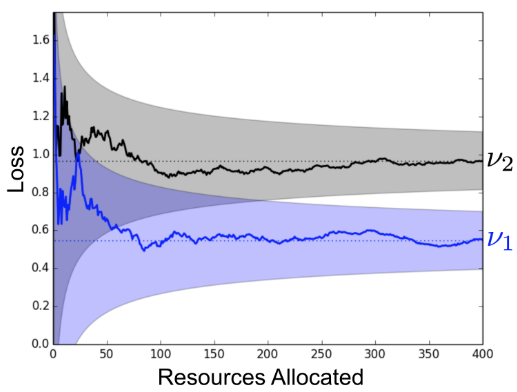
\includegraphics[width=0.95\textwidth]{images/img-004.png}
        \end{column}
    \end{columns}
\end{frame}

\begin{frame}{Hyperband}
    \tiny
    \begin{algorithm}[H]
        \caption{Hyperband for hyperparameter optimization}
        \begin{algorithmic}[1]

            \Require $R, \eta$ (default $\eta = 3$)
            \State $s_{\max} \gets \lfloor \log_\eta(R) \rfloor$
            \State $B \gets (s_{\max} + 1)R$

            \For{$s \in \{s_{\max}, s_{\max} - 1, \dots, 0\}$}
            \State $n \gets \lceil \frac{B}{R} \frac{\eta^s}{(s+1)} \rceil$
            \State $r \gets R \eta^{-s}$

            \State $T \gets \Call{get\_config}{n}$

            \For{$i \in \{0, \dots, s\}$}
            \State $n_i \gets \lfloor n \eta^{-i} \rfloor$
            \State $r_i \gets r \eta^i$
            \State $L \gets \{ \Call{run}{t, r_i} : t \in T \}$ \Comment{Train \& Eval}
            \State $T \gets \Call{top\_k}{T, L, \lfloor n_i/\eta \rfloor}$ \Comment{Keep best}
            \EndFor
            \EndFor

            \State \Return Configuration with smallest loss seen.

        \end{algorithmic}
    \end{algorithm}
\end{frame}

\begin{frame}{Example: LeNet on MNIST}
    \begin{columns}[c]
        \begin{column}{0.5\textwidth}
            \textbf{Setup:}
            \begin{itemize}
                \item Model: LeNet (CNN).
                \item Resource: Iterations (Epochs).
                \item $R=81, \eta=3 \Rightarrow s_{max}=4$.
            \end{itemize}
            \vspace{0.2cm}
            \textbf{Observation:}
            \begin{itemize}
                \item Different brackets ($s$) perform differently.
                \item Hyperband (combining all) is close to the optimal bracket.
            \end{itemize}
        \end{column}
        \begin{column}{0.5\textwidth}
            \centering
            % График сравнения скобок (brackets)
            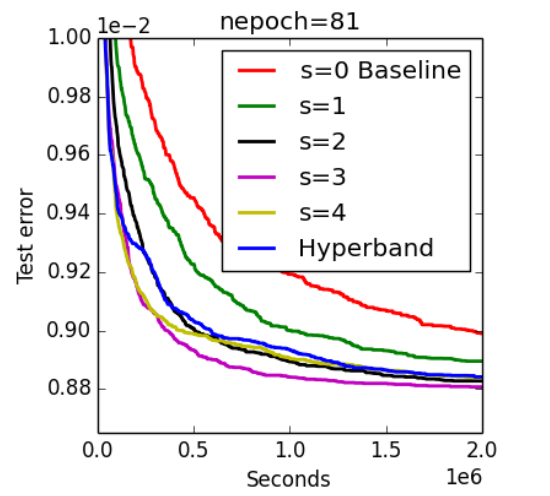
\includegraphics[width=1.0\linewidth]{images/img-006.png}
        \end{column}
    \end{columns}
\end{frame}

\begin{frame}{Exp 1: Deep Learning (Iterations as Resource)}
    \textbf{Task:} CNN tuning on CIFAR-10, MRBI, SVHN.
    \textbf{Resource:} Training Epochs.

    \begin{columns}[T]
        \begin{column}{0.55\textwidth}
            \centering
            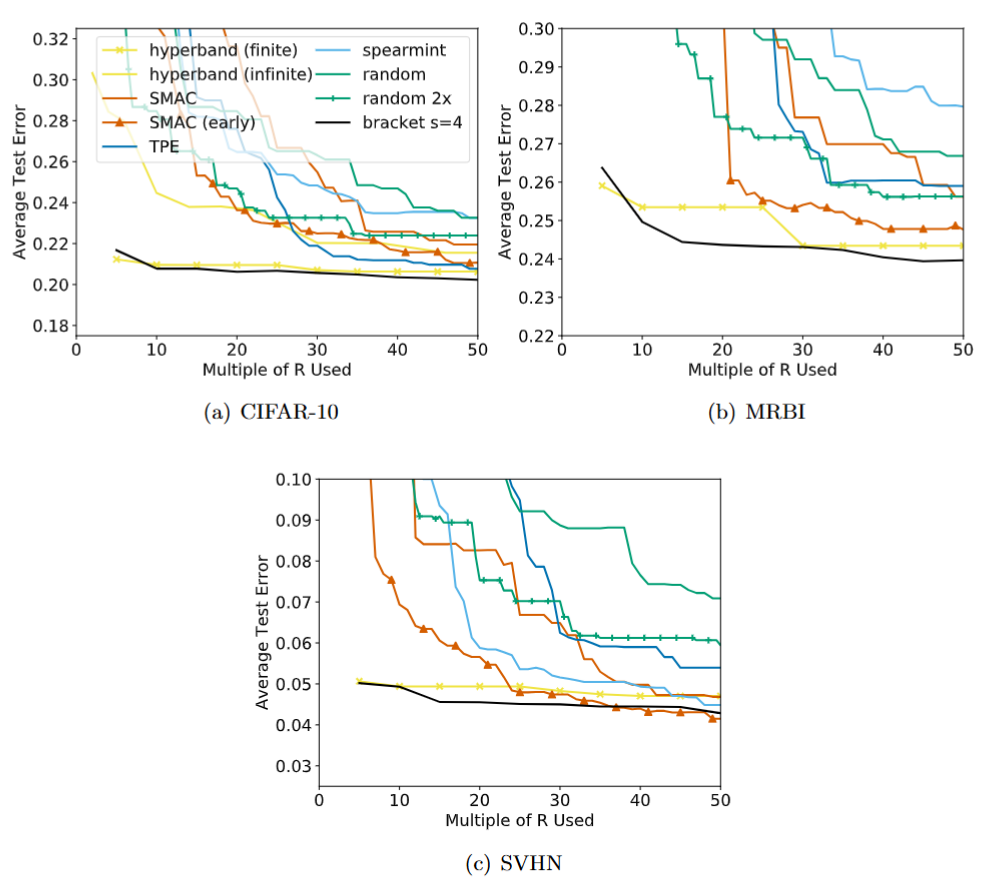
\includegraphics[width=1.0\textwidth, height=0.75\textheight, keepaspectratio]{images/image-deeplearning.png}
        \end{column}
        \begin{column}{0.45\textwidth}
            \vspace{0.5cm}
            \begin{itemize}
                \item \textbf{Result:} Hyperband drops error much faster than Bayesian methods.
                \item \textbf{Speedup:} 5x-30x faster.
                \item Bayesian methods waste time guessing, while Hyperband evaluates hundreds of configs.
            \end{itemize}
        \end{column}
    \end{columns}
\end{frame}

\begin{frame}{Exp 2: Data Subsampling (117 Datasets)}
    \textbf{Task:} Automated ML on 117 OpenML datasets.
    \textbf{Resource:} Subsample size.

    \begin{columns}[T]
        \begin{column}{0.55\textwidth}
            \centering
            % Твоя картинка image-008.png
            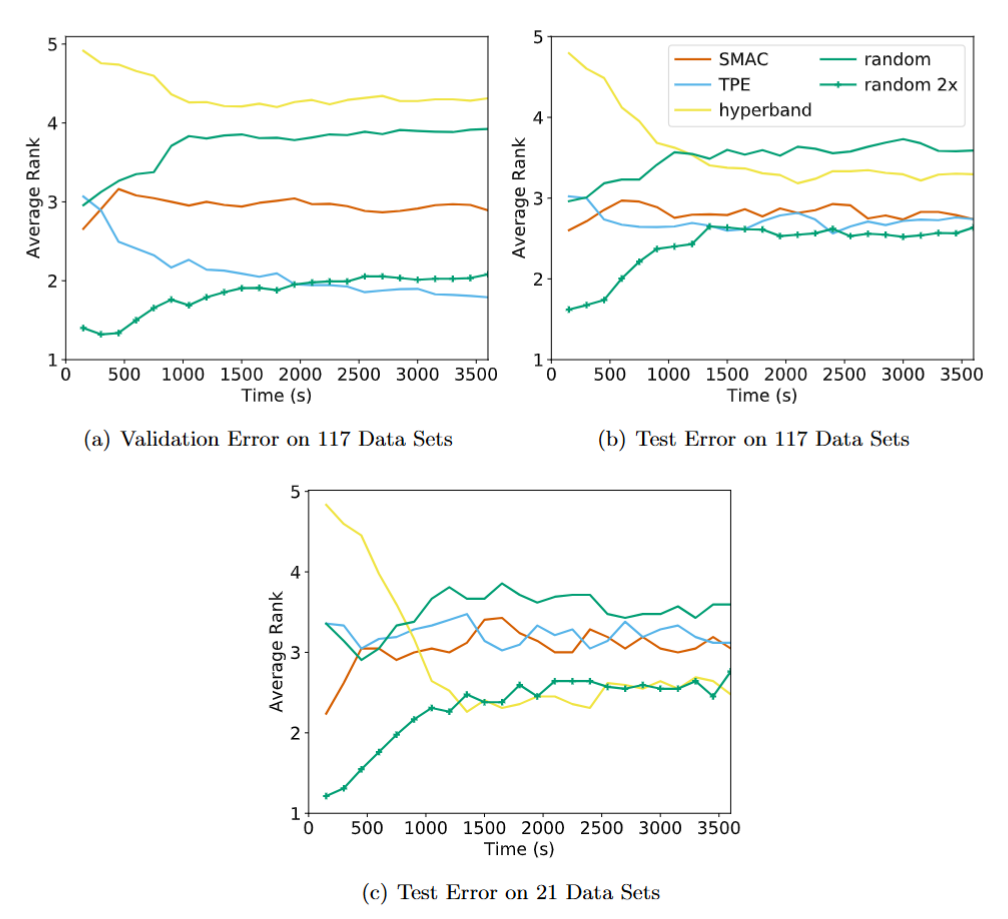
\includegraphics[width=1.0\textwidth, height=0.75\textheight, keepaspectratio]{images/image-openmldatasets.png}
        \end{column}
        \begin{column}{0.45\textwidth}
            \vspace{0.5cm}
            \begin{itemize}
                \item \textbf{Generalization:} Bayesian methods often overfit the validation set.
                \item Hyperband (yellow) performs consistently better on test data.
                \item Effective when subsampling truly reduces computation cost.
            \end{itemize}
        \end{column}
    \end{columns}
\end{frame}

\begin{frame}{Exp 3: Kernel Methods (Non-linear scaling)}
    \textbf{Task:} Kernel Regularized Least Squares (CIFAR-10).
    \textbf{Resource:} Dataset subsample size.

    \begin{columns}[c]
        \begin{column}{0.5\textwidth}
            \centering
            % Твоя картинка image-kernel.png (или image-009 если это она)
            % Вставь правильное имя файла сюда! Я оставил image-009 как плейсхолдер
            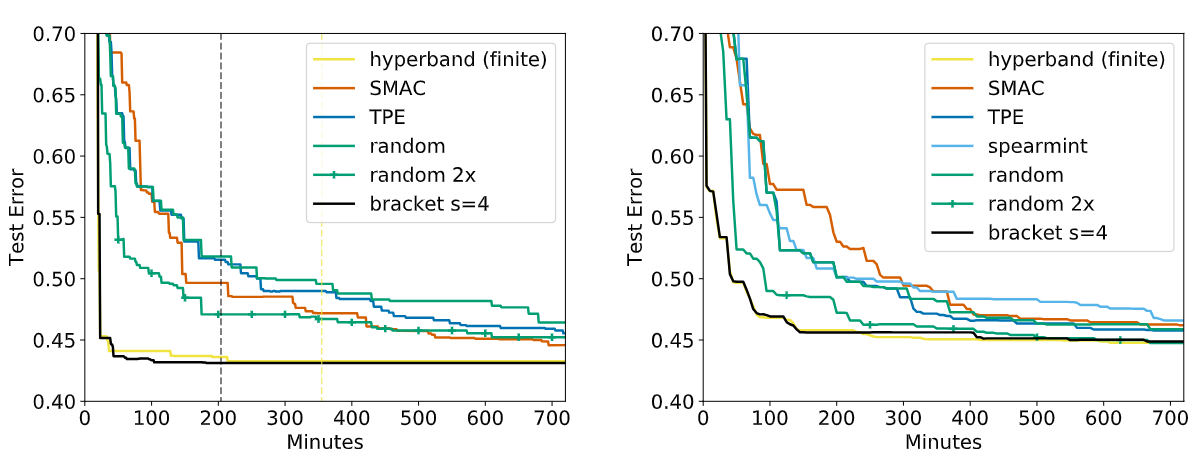
\includegraphics[width=1.0\textwidth, height=0.75\textheight, keepaspectratio]{images/image-kernel.png}
        \end{column}
        \begin{column}{0.5\textwidth}
            \begin{itemize}
                \item Training cost scales as $O(n^3)$.
                \item Evaluating on small subsets is exponentially cheaper.
                \item \textbf{\textcolor{BeaverRed}{70x speedup}} over Random Search.
            \end{itemize}
        \end{column}
    \end{columns}
\end{frame}

\begin{frame}{Conclusion}
    \begin{block}{Key Takeaways}
        \begin{enumerate}
            \item \textbf{Evaluation > Selection:} Allocating resources adaptively is often more efficient than trying to smartly select the next configuration.
            \item \textbf{Robustness:} Hyperband removes the need to manually tune the "exploration vs exploitation" tradeoff ($n$ vs $B/n$).
            \item \textbf{Speed:} 5x to 30x faster than industry-standard Bayesian Optimization methods on Deep Learning tasks.
        \end{enumerate}
    \end{block}
\end{frame}

\end{document}